\documentclass[noauthor,nooutcomes,handout,hints]{ximera}

\graphicspath{  
{./}
{./whoAreYou/}
{./drawingWithTheTurtle/}
{./bisectionMethod/}
{./circles/}
{./anglesAndRightTriangles/}
{./lawOfSines/}
{./lawOfCosines/}
{./plotter/}
{./staircases/}
{./pitch/}
{./qualityControl/}
{./symmetry/}
{./nGonBlock/}
}


%% page layout
\usepackage[cm,headings]{fullpage}
\raggedright
\setlength\headheight{13.6pt}


%% fonts
\usepackage{euler}

\usepackage{FiraMono}
\renewcommand\familydefault{\ttdefault} 
\usepackage[defaultmathsizes]{mathastext}
\usepackage[htt]{hyphenat}

\usepackage[T1]{fontenc}
\usepackage[scaled=1]{FiraSans}

%\usepackage{wedn}
\usepackage{pbsi} %% Answer font


\usepackage{cancel} %% strike through in pitch/pitch.tex


%% \usepackage{ulem} %% 
%% \renewcommand{\ULthickness}{2pt}% changes underline thickness

\tikzset{>=stealth}

\usepackage{adjustbox}

\setcounter{titlenumber}{-1}

%% journal style
\makeatletter
\newcommand\journalstyle{%
  \def\activitystyle{activity-chapter}
  \def\maketitle{%
    \addtocounter{titlenumber}{1}%
                {\flushleft\small\sffamily\bfseries\@pretitle\par\vspace{-1.5em}}%
                {\flushleft\LARGE\sffamily\bfseries\thetitlenumber\hspace{1em}\@title \par }%
                {\vskip .6em\noindent\textit\theabstract\setcounter{question}{0}\setcounter{sectiontitlenumber}{0}}%
                    \par\vspace{2em}
                    \phantomsection\addcontentsline{toc}{section}{\thetitlenumber\hspace{1em}\textbf{\@title}}%
                     }}
\makeatother



%% thm like environments
\let\question\relax
\let\endquestion\relax

\newtheoremstyle{QuestionStyle}{\topsep}{\topsep}%%% space between body and thm
		{}                      %%% Thm body font
		{}                              %%% Indent amount (empty = no indent)
		{\bfseries}            %%% Thm head font
		{)}                              %%% Punctuation after thm head
		{ }                           %%% Space after thm head
		{\thmnumber{#2}\thmnote{ \bfseries(#3)}}%%% Thm head spec
\theoremstyle{QuestionStyle}
\newtheorem{question}{}



\let\freeResponse\relax
\let\endfreeResponse\relax

%% \newtheoremstyle{ResponseStyle}{\topsep}{\topsep}%%% space between body and thm
%% 		{\wedn\bfseries}                      %%% Thm body font
%% 		{}                              %%% Indent amount (empty = no indent)
%% 		{\wedn\bfseries}            %%% Thm head font
%% 		{}                              %%% Punctuation after thm head
%% 		{3ex}                           %%% Space after thm head
%% 		{\underline{\underline{\thmname{#1}}}}%%% Thm head spec
%% \theoremstyle{ResponseStyle}

\usepackage[tikz]{mdframed}
\mdfdefinestyle{ResponseStyle}{leftmargin=1cm,linecolor=black,roundcorner=5pt,
, font=\bsifamily,}%font=\wedn\bfseries\upshape,}


\ifhandout
\NewEnviron{freeResponse}{}
\else
%\newtheorem{freeResponse}{Response:}
\newenvironment{freeResponse}{\begin{mdframed}[style=ResponseStyle]}{\end{mdframed}}
\fi



%% attempting to automate outcomes.

%% \newwrite\outcomefile
%%   \immediate\openout\outcomefile=\jobname.oc
%% \renewcommand{\outcome}[1]{\edef\theoutcomes{\theoutcomes #1~}%
%% \immediate\write\outcomefile{\unexpanded{\outcome}{#1}}}

%% \newcommand{\outcomelist}{\begin{itemize}\theoutcomes\end{itemize}}

%% \NewEnviron{listOutcomes}{\small\sffamily
%% After answering the following questions, students should be able to:
%% \begin{itemize}
%% \BODY
%% \end{itemize}
%% }
\usepackage[tikz]{mdframed}
\mdfdefinestyle{OutcomeStyle}{leftmargin=2cm,rightmargin=2cm,linecolor=black,roundcorner=5pt,
, font=\small\sffamily,}%font=\wedn\bfseries\upshape,}
\newenvironment{listOutcomes}{\begin{mdframed}[style=OutcomeStyle]After answering the following questions, students should be able to:\begin{itemize}}{\end{itemize}\end{mdframed}}



%% my commands

\newcommand{\snap}{{\bfseries\itshape\textsf{Snap!}}}
\newcommand{\flavor}{\link[\snap]{https://snap.berkeley.edu/}}
\newcommand{\mooculus}{\textsf{\textbf{MOOC}\textnormal{\textsf{ULUS}}}}


\usepackage{tkz-euclide}
\tikzstyle geometryDiagrams=[rounded corners=.5pt,ultra thick,color=black]
\colorlet{penColor}{black} % Color of a curve in a plot



\ifhandout\newcommand{\mynewpage}{\newpage}\else\newcommand{\mynewpage}{}\fi


\title{The law of cosines}
\author{Bart Snapp}

\begin{document}
\begin{abstract}
   The law of cosines can help us draw triangles.
\end{abstract}
\maketitle

\begin{listOutcomes}
\item State the law of cosines.
\item Explain why the law of cosines is true.
\item Use the law of cosines to solve a triangle.
\item Use the law of cosines to write a \snap\ block that draws triangles
  based on the SSS congruence theorem.
\item Use the law of cosines to write a \snap\ block that draws triangles
  based on the SAS congruence theorem.
\item Reduce a problem to a previously solved problem.
\item Explain why the converse to the Pythagorean theorem is true.
\item Describe why the converse to the Pythagorean theorem is
  important.
\end{listOutcomes}

Given a triangle
\begin{center}
      \begin{tikzpicture}[geometryDiagrams]
        \coordinate (A) at (0,0);
        \coordinate (B) at (5,2);
        \coordinate (C) at (7,0);
        \tkzDrawSegment (A,B)
        \tkzDrawSegment (A,C)
        \tkzDrawSegment (C,B)
        \tkzLabelSegment[above left](A,B){$c$}
        \tkzLabelSegment[below](A,C){$b$}
        \tkzLabelSegment[above right](B,C){$a$}  

        \tkzMarkAngle[size=1.5cm,thin,mark=](C,A,B)
        \tkzLabelAngle[pos=1.2](C,A,B){$\alpha$}

        \tkzMarkAngle[size=0.8cm,thin,mark=](A,B,C)
        \tkzLabelAngle[pos=.5](A,B,C){$\beta$}

        \tkzMarkAngle[mark=,size=.9,thin](B,C,A)
        \tkzLabelAngle[pos=.6](B,C,A){$\gamma$}
        
      \end{tikzpicture}
\end{center}
the \textbf{law of cosines} states
\[
c^2 = a^2 + b^2 - 2ab\cos(\gamma).
\]
\mynewpage



\begin{question}
  We'll explain WHY the law of cosines is true.
  \begin{enumerate}
    \item Use this picture
      \begin{center}
        \begin{tikzpicture}[geometryDiagrams]
          \coordinate (A) at (0,0);
          \coordinate (B) at (5,2);
          \coordinate (C) at (7,0);
          \tkzDrawSegment (A,B)
          \tkzDrawSegment (A,C)
          \tkzDrawSegment (C,B)
          \tkzLabelSegment[above left](A,B){$c$}
          %\tkzLabelSegment[below](A,C){$b$}
          \tkzLabelSegment[above right](B,C){$a$}  
          
          %\tkzMarkAngle[size=1.5cm,thin,mark=](C,A,B)
          %\tkzLabelAngle[pos=1.2](C,A,B){$\alpha$}
          
          %\tkzMarkAngle[size=0.8cm,thin,mark=](A,B,C)
          %\tkzLabelAngle[pos=.5](A,B,C){$\beta$}
          
          \tkzMarkAngle[mark=,size=.9,thin](B,C,A)
          \tkzLabelAngle[pos=.6](B,C,A){$\gamma$}
          \tkzDrawLine[altitude](A,B,C)\tkzGetPoint{D}
          \tkzMarkRightAngle[thin](B,D,C)
          \tkzLabelSegment[left](D,B){$h$}
          \tkzLabelSegment[below](A,D){$e$}
          \tkzLabelSegment[below](C,D){$d$}
        \end{tikzpicture}
      \end{center}
      to explain why:
      \begin{align*}
        h &= a\cdot \sin(\gamma)\\
        d &= a\cdot \cos(\gamma) \\
        e &= b - a\cdot \cos(\gamma)
      \end{align*}
    \item Now substitute/expand
      \[
      c^2 = h^2 + e^2
      \]
      to conclude:
      \[
      c^2 = a^2 + b^2 - 2ab\cos(\gamma)
      \]
      \begin{hint}
        Recall that $\cos^2(\theta) + \sin^2(\theta) = 1$.
      \end{hint}
  \end{enumerate}
\end{question}
\mynewpage

\begin{question}
  Let's build some \snap\ blocks!
  \begin{enumerate}
  \item Create a \snap\ block that will draw triangles based on the
    SSS congruence theorem.  As a gesture of friendship, I've started
    the block for you:
    \begin{center}
      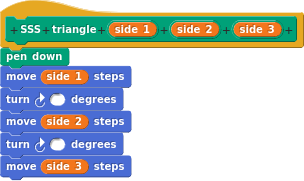
\includegraphics{sssBlockBLANK}
    \end{center}
    It's your job to USE THE LAW OF COSINES to fill in the
    blanks. EXPLAIN how you used the law of cosines, and show off your
    work by giving screenshots of your SCRIPT and STAGE as provided
    from \snap.
  \item Use your work from the previous part to create a \snap\ block
    that will draw triangles based on the SAS congruence theorem.  As
    a gesture of friendship, I've started the block for you:
    \begin{center}
      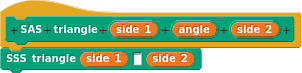
\includegraphics{sasBlockBLANK}
    \end{center}
    It's your job to USE THE LAW OF COSINES to fill in the
    blank.
  \end{enumerate}
    In EACH case above, EXPLAIN how you used the law of cosines, and
    show off your work by giving screenshots of your SCRIPT and STAGE
    as provided from \snap.
    \begin{freeResponse}
      \begin{enumerate}
      \item Consider this triangle:
        \begin{center}
          \begin{tikzpicture}[geometryDiagrams]
            \coordinate (A) at (0,0);
            \coordinate (B) at (5,2);
            \coordinate (C) at (7,0);
            \tkzDrawSegment (A,B)
            \tkzDrawSegment (A,C)
            \tkzDrawSegment (C,B)
            \tkzLabelSegment[above left](A,B){$side~1$}
            \tkzLabelSegment[below](A,C){$side~3$}
            \tkzLabelSegment[above right](B,C){$side~2$}  
          
            %\tkzMarkAngle[size=1.5cm,thin,mark=](C,A,B)
            %\tkzLabelAngle[pos=1.2](C,A,B){$\alpha$}
          
            \tkzMarkAngle[size=0.8cm,thin,mark=](A,B,C)
            \tkzLabelAngle[pos=.5](A,B,C){$\theta$}
            
          %% \tkzMarkAngle[mark=,size=.9,thin](B,C,A)
            %% \tkzLabelAngle[pos=.6](B,C,A){$\gamma$}
            
          \end{tikzpicture}
        \end{center}
        Note by the law of cosines:
        \[
        (\mathrm{side~3})^2 = (\mathrm{side~1})^2 + (\mathrm{side~2})^2 - 2\cdot (\mathrm{side~1})(\mathrm{side~2})\cos(\theta)
        \]
        Hence the angle between $\mathrm{side~1}$ and $\mathrm{side~2}$ is given by:
        \[
        \theta = \arccos\left(\frac{(\mathrm{side~1})^2 + (\mathrm{side~2})^2- (\mathrm{side~3})^2}{2\cdot (\mathrm{side~1})(\mathrm{side~2})})\right) 
        \]
        This is the first angle we need for our script.
        
        Now consider this triangle:
        \begin{center}
          \begin{tikzpicture}[geometryDiagrams]
            \coordinate (A) at (0,0);
            \coordinate (B) at (5,2);
            \coordinate (C) at (7,0);
            \tkzDrawSegment (A,B)
            \tkzDrawSegment (A,C)
            \tkzDrawSegment (C,B)
            \tkzLabelSegment[above left](A,B){$side~1$}
            \tkzLabelSegment[below](A,C){$side~3$}
            \tkzLabelSegment[above right](B,C){$side~2$}  
            
            %\tkzMarkAngle[size=1.5cm,thin,mark=](C,A,B)
            %\tkzLabelAngle[pos=1.2](C,A,B){$\alpha$}
          
            %\tkzMarkAngle[size=0.8cm,thin,mark=](A,B,C)
            %\tkzLabelAngle[pos=.5](A,B,C){$\theta$}
            
            \tkzMarkAngle[mark=,size=.9,thin](B,C,A)
            \tkzLabelAngle[pos=.6](B,C,A){$\theta$}
            
        \end{tikzpicture}
        \end{center}
        Note by the law of cosines:
        \[
        (\mathrm{side~1})^2 = (\mathrm{side~2})^2 + (\mathrm{side~3})^2 - 2\cdot (\mathrm{side~2})(\mathrm{side~3})\cos(\theta)
        \]
        Hence the angle between $\mathrm{side~1}$ and $\mathrm{side~2}$ is given by:
        \[
        \theta = \arccos\left(\frac{(\mathrm{side~2})^2 + (\mathrm{side~3})^2- (\mathrm{side~1})^2}{2\cdot (\mathrm{side~2})(\mathrm{side~3})})\right) 
        \]
        This is the the second angle we need for our script.
        Here is my script and my stage:
        \begin{center}
          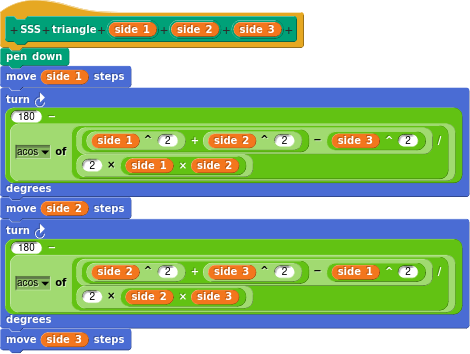
\includegraphics[width=.4\textwidth]{sssBlockCOMPLETE}   \qquad \fbox{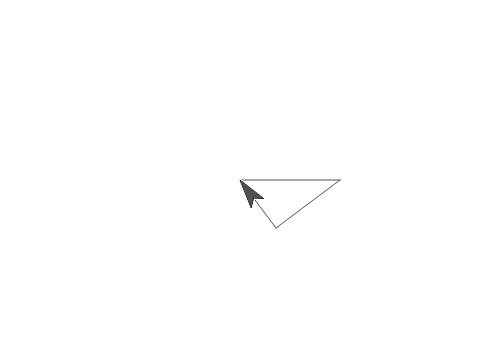
\includegraphics[width=.4\textwidth]{sssStage.png}}
        \end{center}
      \item Consider this triangle:
    \begin{center}
        \begin{tikzpicture}[geometryDiagrams]
          \coordinate (A) at (0,0);
          \coordinate (B) at (5,2);
          \coordinate (C) at (7,0);
          \tkzDrawSegment (A,B)
          \tkzDrawSegment (A,C)
          \tkzDrawSegment (C,B)
          \tkzLabelSegment[above left](A,B){$side~1$}
          \tkzLabelSegment[below](A,C){$side~3$}
          \tkzLabelSegment[above right](B,C){$side~2$}  
          
          %\tkzMarkAngle[size=1.5cm,thin,mark=](C,A,B)
          %\tkzLabelAngle[pos=1.2](C,A,B){$\alpha$}
          
          \tkzMarkAngle[size=0.8cm,thin,mark=](A,B,C)
          \tkzLabelAngle[pos=.5](A,B,C){$\theta$}
          
          %% \tkzMarkAngle[mark=,size=.9,thin](B,C,A)
          %% \tkzLabelAngle[pos=.6](B,C,A){$\gamma$}
          
        \end{tikzpicture}
      \end{center}
    Now we can find the third side via the law of cosines
    \[
    (\mathrm{side~3})^2 = (\mathrm{side~1})^2 + (\mathrm{side~2})^2 - 2\cdot (\mathrm{side~1})(\mathrm{side~2})\cos(\theta)
    \]
    so
    \[
    side~3= \sqrt{(\mathrm{side~1})^2 + (\mathrm{side~2})^2 - 2\cdot (\mathrm{side~1})(\mathrm{side~2})\cos(\theta)}.
    \]
    Now that we know the three sides, we can use our previous block.
    Here is my script and my stage:
    \begin{center}
      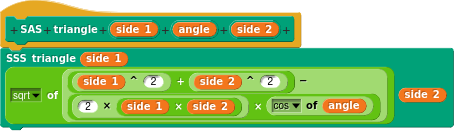
\includegraphics[width=.4\textwidth]{sasBlockCOMPLETE}   \qquad \fbox{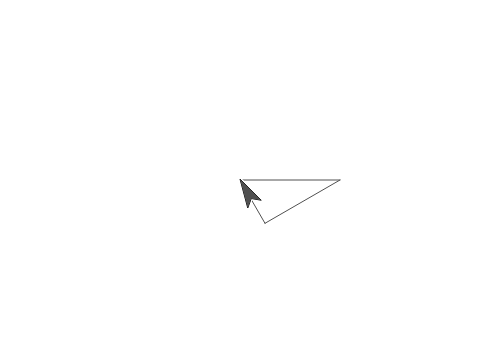
\includegraphics[width=.4\textwidth]{sasStage.png}}
    \end{center}
      \end{enumerate}
\end{freeResponse}
\end{question}
\mynewpage



\begin{question}
  Perhaps, more important than the Pythagorean theorem is the:
  \begin{quote}
    \textbf{Converse to the Pythagorean theorem}:
    Suppose that I have three positive numbers $a$, $b$, and $c$ such that:
    \[
    a^2 + b^2 = c^2
    \]
    In this case, there exists a right triangle with legs $a$ and $b$
    and hypotenuse $c$.
  \end{quote}
  \begin{enumerate}
  \item Explain WHY the converse to the Pythagorean theorem is true.
    \begin{hint}
      Think SAS. 
    \end{hint}
  \item Explain WHY someone might think that the CONVERSE to the
    Pythagorean theorem is MORE IMPORTANT than the Pythagorean
    theorem.
  \end{enumerate}
    \begin{freeResponse}
      \begin{enumerate}
      \item Well as long as all of $a$, $b$, and $c$ are positive numbers there
        will be such a triangle, by SAS.  One side has length $a$, the
        other has length $b$, and the angle is the right angle between
        them. Since there is only one such triangle, and it's a right
        triangle, the Pythagorean theorem guarantees that the final side
        must have length $c = \sqrt{a^2+b^2}$.
      \item The CONVERSE to the Pythagorean theorem is MORE IMPORTANT
        than the Pythagorean theorem because it gives us an easy way
        to identify if an angle is right angle, simply by measuring
        sides.
      \end{enumerate}
      \end{freeResponse}
  
\end{question}


\end{document}
